\section{Bifurcations}
\label{sec:dynarch.bif}
\label{sec:minrep.bif}

This section lists the bifurcations that happen at the borders of ``type A'' and ``type B'' parameter regions, respectively.
\Cref{fig:final.regions.whole.halved} shows the borders of the period regions in full.
%\Cref{fig:final.regions.EandF16.halved} is a zoomed-in version, that pictures the two regions that this section investigates.
%These two regions are $\P_{\A^5\B^3C^5\D^3}$, which is the parameter region that includes the point $E_{16}$, and $\P_{\A^5\B^3\C^4\D^4, \A^4\B^4\C^5\D^3}$, which includes the point $F_{16}$.
%The arrows in that figure mark, where the bifurcation diagrams in this section are computed.
\Cref{fig:final.regions.F16.halved} is a zoomed-in verions, that pictures the region that this section investigates the boundaries of.
It is the parameter region that include the point $F_{16}$ pictured in \Cref{fig:final.period.whole.halved}, $\P_{\A^5\B^3\C^4\D^4, \A^4\B^4\C^5\D^3}$.
As we can see from the coexisting cycles $\Cycle{\A^5\B^3\C^4\D^4}$ and $\Cycle{\A^4\B^4\C^5\D^3}$, this is a ``type B'' parameter region.
Every one of its boundaries has a ``type A'' parameter region on the other side.
Therefore, we only need to describe the 4 boundaries of this ``type B'' parameter region in depth to cover the boundaries of both ``type A'' and ``type B'' parameter regions.

\begin{figure}
	\centering
	\subfloat[Complete parameter region]{
		\includegraphics[width=.4\textwidth]{60_MinimalRepr/2D_Regions_Whole/result-halved.png}
		\label{fig:final.regions.whole.halved}
	}
	%    \begin{subfigure}{0.4\textwidth}
	%        \centering
	%        \includegraphics[width=\textwidth]{60_MinimalRepr/2D_Regions_EandF16/result-halved.png}
	%        \caption{Only showing $E_{16}$ and $F_{16}$}
	%        \label{fig:final.regions.EandF16.halved}
	%    \end{subfigure}
	\subfloat[Only showing the parameter region including the point $F_{16}$]{
		\includegraphics[width=.4\textwidth]{60_MinimalRepr/2D_Regions_F_Boundaries/result.png}
		\label{fig:final.regions.F16.halved}
	}
	\caption{2D period regions of the halved final model}
\end{figure}

%\subsection{``Type A'' Parameter Regions}

%We start with the bifurcations bounding the ``type A'' parameter region containing the point $E_{16}$, $\P_{\A^5\B^3\C^5\D^3}$.
%The boundaries are referred to as $E_{16}^\uparrow, E_{16}^\rightarrow, E_{16}^\downarrow,$ and $E_{16}^\leftarrow$, where the arrow in the superscript indicates the side of the border.
%So $E_{16}^\uparrow$ means the upper border of the period region, that contains the point $E_{16}$.

%\subsubsection{The Boundary $E_{16}^\uparrow$}
%\label{sec:final.bifurcation.typeA.up}

%When scanning across the upper boundary of this parameter region, one gets the figure \Cref{fig:final.bifurcation.E.up}.
%It is not immediately clear, what kind of bifurcation happens.
%The bifurcation diagram has to be read from left to right, this is also true for all other bifurcation diagrams in this section.
%It does not show the stable cycle of the next parameter region above $\P_{\A^5\B^3\C^5\D^3}$ while the stable cycle $\A^5\B^3\C^5\D^3$ still exists.
%We are interested in what happens to this stable cycle that exists at the start and causes it to vanish.
%The cycle is near the border $d_1$ when it vanishes, so we can zoom into that area.
%It is marked black in the bifurcation diagram and pictured in \Cref{fig:bifurcation.E.up.zoomed}.
%It is immediately clear, that this is a border bifurcation with the stable cycle $\Cycle{\A^5\B^3\C^5\D^3}$ colliding with the border $d_1$ from the left side, meaning one point of the cycle on the branch $\Branch_\A$ collides with this border.
%Analogous, a point of this cycle on branch $\C$ collides with the border $d_3$ because of the symmetry of our function.
%We will write $\BCB_{d_1, d_3}^{\A^5\B^3\C^5\D^3, r}$, which means that this is a border bifurcation at the border $d_1$ and $d_3$ where the points collide from the left (branches $\Branch_\A$ and $\Branch_\C$ respectively).

%\begin{figure}
%    \centering
%    \begin{subfigure}{0.4\textwidth}
%        \centering
%        \includegraphics[width=\textwidth]{60_MinimalRepr/1D_Bif_LEU16/result.png}
%        \caption{Complete}
%        \label{fig:final.bifurcation.E.up}
%    \end{subfigure}
%    \begin{subfigure}{0.4\textwidth}
%        \centering
%        \includegraphics[width=\textwidth]{60_MinimalRepr/1D_Bif_LEU16_Zoomed/result.png}
%        \caption{Zoomed-in at Border $d_1$}
%        \label{fig:bifurcation.E.up.zoomed}
%    \end{subfigure}
%    \caption{1D Bifurcation Diagrams of $E_{16}^\uparrow$}
%\end{figure}

%\subsubsection{The Boundary $E_{16}^\rightarrow$}

%Taking a look at the right boundary of this parameter region, we get the bifurcation diagram in \Cref{fig:final.bifurcation.E.right}.
%This time, the stable cycle existing at the start is nowhere near the borders $d_1$ or $d_3$ when it vanishes.
%Instead, it is near the border $d_2$ and $d_0$ respectively.
%Zooming into the marked region again, we get \Cref{fig:final.bifurcation.E.right.zoomed}.
%From these bifurcation diagrams, we can conclude that the bifurcation at this boundary is $\BCB_{d_0, d_2}^{\A^5\B^3\C^5\D^3, l}$.

%\begin{figure}
%    \centering
%    \begin{subfigure}{0.4\textwidth}
%        \centering
%        \includegraphics[width=\textwidth]{60_MinimalRepr/1D_Bif_LER16/result.png}
%        \caption{Complete}
%        \label{fig:final.bifurcation.E.right}
%    \end{subfigure}
%    \begin{subfigure}{0.4\textwidth}
%        \centering
%        \includegraphics[width=\textwidth]{60_MinimalRepr/1D_Bif_LER16_Zoomed/result.png}
%        \caption{Zoomed-in at Border $d_2$}
%        \label{fig:final.bifurcation.E.right.zoomed}
%    \end{subfigure}
%    \caption{1D Bifurcation Diagrams of $E_{16}^\rightarrow$}
%\end{figure}

%\subsubsection{The Boundary $E_{16}^\downarrow$}

%\Cref{fig:final.bifurcation.E.down} shows the bifurcation diagram for the lower boundary of the parameter region $\P_{\A^5\B^3\C^5\D^3}$.
%We can see, that the stable cycle is near the borders $d_1$ and $d_3$ when it vanishes.
%\Cref{fig:final.bifurcation.E.down.zoomed} shows the zoomed-in region marked black in the full bifurcation diagram \Cref{fig:final.bifurcation.E.down}.
%From these bifurcation diagrams, we can conclude that the bifurcation at this boundary is $\BCB_{d_1, d_3}^{\A^5\B^3\C^5\D^3, l}$

%\begin{figure}
%    \centering
%    \begin{subfigure}{0.4\textwidth}
%        \centering
%        \includegraphics[width=\textwidth]{60_MinimalRepr/1D_Bif_LED16/result.png}
%        \caption{Complete}
%        \label{fig:final.bifurcation.E.down}
%    \end{subfigure}
%    \begin{subfigure}{0.4\textwidth}
%        \centering
%        \includegraphics[width=\textwidth]{60_MinimalRepr/1D_Bif_LED16_Zoomed/result.png}
%        \caption{Zoomed-in at Border $d_1$}
%        \label{fig:final.bifurcation.E.down.zoomed}
%    \end{subfigure}
%    \caption{1D Bifurcation Diagrams of $E_{16}^\downarrow$}
%\end{figure}

%\subsubsection{The Boundary $E_{16}^\leftarrow$}

%Similarly, \Cref{fig:final.bifurcation.E.left} shows the bifurcation diagram at the lower boundary of the parameter region $\P_{\A^5\B^3\C^5\D^3}$.
%The stable cycle is near the borders $d_0$ and $d_2$ when it vanishes and \Cref{fig:final.bifurcation.E.left.zoomed} shows a zoomed-in version of the bifurcation diagram.
%The region that is depicted in the zoomed-in version is marked black in \Cref{fig:final.bifurcation.E.left}.
%From these bifurcation diagrams, we can conclude that the bifurcation at this boundary is $\BCB_{d_0, d_2}^{\A^5\B^3\C^5\D^3, r}$.

%\begin{figure}
%    \centering
%    \begin{subfigure}{0.4\textwidth}
%        \centering
%        \includegraphics[width=\textwidth]{60_MinimalRepr/1D_Bif_LEL16/result.png}
%        \caption{Complete}
%        \label{fig:final.bifurcation.E.left}
%    \end{subfigure}
%    \begin{subfigure}{0.4\textwidth}
%        \centering
%        \includegraphics[width=\textwidth]{60_MinimalRepr/1D_Bif_LEL16_Zoomed/result.png}
%        \caption{Zoomed-in at Border $d_2$}
%        \label{fig:final.bifurcation.E.left.zoomed}
%    \end{subfigure}
%    \caption{1D Bifurcation Diagrams of $E_{16}^\leftarrow$}
%\end{figure}

%\subsection{``Type B'' Parameter Regions}

%This section covers the bifurcations happening at the bounds of ``type B'' parameter regions.
%For this purpose, we consider the parameter region $\P_{\A^5\B^3\C^4\D^4, \A^4\B^4\C^5\D^3}$ that contains the point $F_{16}$.
%In contrast to the last section covering ``type A'' parameter regions, here there are two coexisting stable cycles.
%The boundaries are enumerated as $F_{16}^\uparrow, F_{16}^\rightarrow, F_{16}^\downarrow,$ and $F_{16}^\leftarrow$.

\subsubsection{The Boundary $F_{16}^\uparrow$}
\label{sec:minrep.bif.U}

\Cref{fig:final.bifurcation.F.up} shows the bifurcation diagram of the first considered border, $F_{16}^\uparrow$.
The two existing stable cycles at the beginning are drawn in different colors to differentiate them.
The cycle $\Cycle{\A^5\B^3\C^4\D^4}$ is green and its rotated twin $\Cycle{\A^4\B^4\C^5\D^3}$ is red.
One can see that the green cycle collides with the border $d_1$ when it vanishes.
To be more precise the point $x_4^{\A^5\B^3\C^4\D^4}$, which is the 5th point of the cycle $\Cycle{\A^5\B^3\C^4\D^4}$, collides with the border $d_1$.
This bifurcation is denoted as $\BCB_{d_1}^{\A^5\B^3\C^4\D^4}$.
The same thing happens to its rotated twin, the red cycle at the border $d_3$ because of the symmetry.
Here, the point $x_{12}^{A^4\B^4\C^5\D^3}$ collides with the border $d_3$ and the bifurcation is denoted as $\BCB_{d_3}^{A^4\B^4\C^5\D^3}$.
In both cases, the cycles collide from the left side of the border, so for $\Cycle{\A^5\B^3\C^4\D^4}$, one point of the cycle on branch $f_{\A}$ collided with the border $d_1$.
And analogous, for $\Cycle{\A^4\B^4\C^5\D^3}$, one point of the cycle on the branch $f_{\C}$ collided with the border $d_3$.

The ``type A'' parameter region above is $\P_{\A^4\B^4\C^4\D^4}$.
The cycle $\Cycle{\A^4\B^4\C^4\D^4}$ (blue), which is stable in that parameter region, also collides with the same borders, the cycles $\Cycle{\A^5\B^3\C^4\D^4}$ and $\Cycle{\A^4\B^4\C^5\D^3}$ from the ``type B'' parameter region collided with, $d_1$ and $d_3$.
But here, two points of the same cycle collide with two different borders at the same parameter values.
Point $x_{4}^{A^4\B^4\C^4\D^4}$ collides with the border $d_1$ while point $x_{12}^{A^4\B^4\C^4\D^4}$ collides with $d_3$, both from below.
So one point of the cycle on the branch $f_{\B}$ collides with $d_1$ and one point on the branch $f_{\D}$ collides with $d_3$.
This is unusual for border collision bifurcations but is explained by the symmetry of both the cycle and the function.
The bifurcation is denoted as $\BCB_{d_1, d_3}^{\A^4\B^4\C^4\D^4}$.

\begin{figure}
	\centering
	\includegraphics[width=.7 \textwidth]{60_MinimalRepr/1D_Bif_LFU16/Manual/result.png}
	\label{fig:final.bifurcation.F.up}
	\caption{1D bifurcation diagram at the boundary $F_{16}^\uparrow$}
\end{figure}

\subsubsection{The Boundary $F_{16}^\downarrow$}
\label{sec:minrep.bif.D}

At the lower boundary $F_{16}^\downarrow$, the two cycles $\Cycle{\A^5\B^3\C^4\D^4}$ and $\Cycle{\A^4\B^4\C^5\D^3}$ also collide with the borders $d_1$ and $d_3$, this time from above rather than from below.
But while the cycle $\Cycle{\A^5\B^5\C^4\D^4}$ collided with the border $d_1$ at the upper boundary, it now collides with the border $d_3$.
To be more precise, the point $x_{12}^{\A^5\B^3\C^4\D^4}$ collides with the border $d_3$ meaning one point on the branch $f_{\D}$ collides with the border $d_3$.
Analogous, the point $x_{4}^{\A^4\B^4\C^5\D^3}$ of the cycle $\Cycle{\A^4\B^4\C^5\D^3}$ now collides with the border $d_1$ from above.
Meaning that one point of branch $f_{\B}$ collides with the border $d_1$. The bifurcations are denoted as $\BCB_{d_3}^{\A^5\B^3\C^4\D^4}$ and $\BCB_{d_1}^{\A^4\B^4\C^5\D^3}$.

The ``type A'' parameter region below is $\P_{\A^5\B^3\C^5\D^3}$.
The cycle $\P_{\A^5\B^3\C^5\D^3}$, pictured in blue, collides with the same borders, just like before at the upper boundary.
Again, two points of this cycle collide with two different borders, $d_1$ and $d_2$ at the same parameter values, but this time from below.
The point colliding with $d_1$ is $x_{4}^{A^5\B^3\C^5\D^3}$ and  the point colliding with $d_3$ is $x_{12}^{A^5\B^3\C^5\D^3}$.
So one point on the branch $f_{\A}$ collides with the border $d_1$ and one point on the branch $f_{\C}$ collides with the border $d_3$.
This bifurcation is denoted as $\BCB_{d_1, d_3}^{\A^5\B^3\C^5\D^3}$.

\todo{is the following paragraph fitting?}
It is as if the ``type A'' and ``type B'' cycles switched roles from the $F_{16}^\uparrow$ boundary to this $F_{16}^\downarrow$ boundary.
The cycles collide with the same borders, but the side from which they collide are swapped.

\begin{figure}
	\centering
	\includegraphics[width=.7 \textwidth]{60_MinimalRepr/1D_Bif_LFD16/Manual/result.png}
	\label{fig:final.bifurcation.F.down}
	\caption{1D bifurcation diagram at the boundary $F_{16}^\downarrow$}
\end{figure}

\subsubsection{The Boundary $F_{16}^\rightarrow$}
\label{sec:minrep.bif.R}

Now we will take a look at the horizontal boundaries of this ``type B'' parameter region.
At the right boundary $F_{16}^\rightarrow$, the two cycles $\Cycle{\A^5\B^3\C^4\D^4}$ and $\Cycle{\A^4\B^4\C^5\D^3}$ collide with the borders $d_0$ and $d_2$ from above.
These are different borders from before at the boundaries $F_{16}^\uparrow$ and $F_{16}^\downarrow$.
The first point of cycle $\Cycle{A^4B^4\C^5\D^3}$, $x_{0}^{\A^4\B^4\C^5\D^3}$ collides with the boundary $d_0$, while the point $x_{8}^{\A^5\B^3\C^4\D^4}$ from its twin cycle $\Cycle{\A^5\B^3\C^4\D^4}$ collides with the border $d_2$.
This means that one point of the cycle $\Cycle{\A^4\B^4\C^5\D^3}$ on the branch $f_{\A}$ collides with the border $d_0$ and one point of the cycle $\Cycle{\A^5\B^3\C^4\D^4}$ on the branch $f_{\C}$ collides with the border $d_2$.
The bifurcations are denoted as $\BCB_{d_0}^{\A^4\B^4\C^5\D^3}$ and $\BCB_{d_2}^{\A^5\B^3\C^4\D^4}$ respectively.

The parameter region right to this parameter region is $\P_{\A^5\B^4\C^5\D^4}$.
As before with the vertical boundaries $f_{16}^\uparrow$ and $F_{16}^\downarrow$, the cycle of the neighboring ``type A'' parameter region collides with the same borders as the cycles of the ``type B'' but from the opposite direction.
In this case, two of the points of the cycle $\Cycle{\A^5\B^4\C^5\D^4}$ collide with the borders $d_0$ and $d_1$ at the same parameter value from below.
To be more precise, the point $x_{17}^{\A^5\B^4\C^5\D^4}$, which is on the branch $f_{\D}$, collides with the border $d_0$ while the point $x_{8}^{\A^5\B^4\C^5\D^4}$, which is on the branch $f_{\B}$, collides with the border $d_2$.
This bifurcation is denoted as $\BCB_{d_0, d_2}^{\A^5\B^4\C^5\D^4}$.

\begin{figure}
	\centering
	\includegraphics[width=.7 \textwidth]{60_MinimalRepr/1D_Bif_LFR16/Manual/result.png}
	\label{fig:final.bifurcation.F.right}
	\caption{1D bifurcation diagram at the boundary $F_{16}^\rightarrow$}
\end{figure}

\subsubsection{The Boundary $F_{16}^\leftarrow$}
\label{sec:minrep.bif.L}

At the left boundary $F_{16}^\leftarrow$, the two cycles $\Cycle{\A^5\B^3\C^4\D^4}$ and $\Cycle{\A^4\B^4\C^5\D^3}$ collide with the same borders as before, but this time from below.
The point $x_{7}^{\A^4\B^4\B^5\D^3}$, which is on branch $f_{\B}$, collides with $d_2$ while the point $x_{15}^{\A^5\B^3\C^4\D^4}$, which is on branch $f_{\D}$, colides with the border $d_0$.
These bifurcations are denoted $\BCB_{d_0}^{\A^5\B^3\C^4\D^4}$ and $\BCB_{d_2}^{\A^4\B^4\C^5\D^3}$ respectively.

The parameter region left to this parameter region is $\P_{\A^4\B^3\C^4\D^3}$.
Here again, the cycle of the ``type A'' parameter region collides with the same borders, as the cycles of the ``type B'' parameter region collided with, $d_0$ and $d_2$ from the opposing direction.
The point $x_{0}^{\A^4\B^3\C^4\D^3}$, which is on branch $f_{\A}$, colides with the border $d_0$ while the point $x_{7}^{\A^4\B^3\C^4\D^3}$, which is on branch $f_{\C}$, collides with the border $d_2$.
This bifurcation is denoted as $\BCB_{d_0, d_2}^{\A^4\B^3\C^4\D^3}$.

Just like with the vertical boundaries, $F_{16}^\uparrow$ and $F_{16}^\downarrow$, we can observe that the cycles seem to switch roles at the two boundaries $F_{16}^\rightarrow$ and $F_{16}^\leftarrow$.
\todo{expand if section makes sense}

\begin{figure}
	\centering
	\includegraphics[width=.7 \textwidth]{60_MinimalRepr/1D_Bif_LFL16/Manual/result.png}
	\label{fig:final.bifurcation.F.left}
	\caption{1D bifurcation diagram at the boundary $F_{16}^\leftarrow$}
\end{figure}

\todo{summarize rules for bifurcations in either type of parameter region, like akyuz}

%\subsection{Listing the Bifurcations}

%\begin{table}
%    \centering
%    \begin{tabular}{| l || c | c |}
%        \hline
%                      & $E_{16}$                                & $F_{16}$                                                                  \\ \hline \hline
%        $\uparrow$    & $\BCB_{d_1, d_3}^{\A^5\B^3\C^5\D^3, r}$ & $\BCB_{d_1}^{\A^5\B^3\C^4\D^4, r}$ and $\BCB_{d_3}^{\A^4\B^4\C^5\D^3, r}$ \\ \hline
%        $\rightarrow$ & $\BCB_{d_0, d_2}^{\A^5\B^3\C^5\D^3, l}$ & $\BCB_{d_2}^{\A^5\B^3\C^4\D^4, l}$ and $\BCB_{d_0}^{\A^4\B^4\C^5\D^3, l}$ \\ \hline
%        $\downarrow$  & $\BCB_{d_1, d_3}^{\A^5\B^3\C^5\D^3, l}$ & $\BCB_{d_3}^{\A^5\B^3\C^4\D^4, l}$ and $\BCB_{d_1}^{\A^4\B^4\C^5\D^3, l}$ \\ \hline
%        $\leftarrow$  & $\BCB_{d_0, d_2}^{\A^5\B^3\C^5\D^3, r}$ & $\BCB_{d_0}^{\A^5\B^3\C^4\D^4, r}$ and $\BCB_{d_2}^{\A^4\B^4\C^5\D^3, r}$ \\ \hline
%    \end{tabular}
%    \caption{Table of the Bifurcations}
%\end{table}
